\documentclass{article}

% Packages for formatting
\usepackage[margin=1in]{geometry}
\usepackage{fancyhdr}
\usepackage{enumerate}
\usepackage{graphicx}
\usepackage{kotex}
\usepackage{amsmath}
\usepackage{amsthm}
\usepackage{algorithm2e,setspace}
\usepackage{algpseudocode}
\usepackage{xcolor}
\usepackage{amssymb}

% Fonts
\usepackage[T1]{fontenc}
\usepackage[utf8]{inputenc}
\usepackage{newpxtext,newpxmath}
\usepackage{sectsty}

% Define colors
\definecolor{blue1}{HTML}{0077c2}
\definecolor{blue2}{HTML}{00a5e6}
\definecolor{blue3}{HTML}{b3e0ff}
\definecolor{blue4}{HTML}{00293c}
\definecolor{blue5}{HTML}{e6f7ff}

\definecolor{thmcolor}{RGB}{231, 76, 60}
\definecolor{defcolor}{RGB}{52, 152, 219}
\definecolor{lemcolor}{RGB}{155, 89, 182}
\definecolor{corcolor}{RGB}{46, 204, 113}
\definecolor{procolor}{RGB}{241, 196, 15}

\usepackage{color,soul}
\usepackage{soul}
\newcommand{\mathcolorbox}[2]{\colorbox{#1}{$\displaystyle #2$}}
\usepackage{cancel}
\newcommand\crossout[3][black]{\renewcommand\CancelColor{\color{#1}}\cancelto{#2}{#3}}
\newcommand\ncrossout[2][black]{\renewcommand\CancelColor{\color{#1}}\cancel{#2}}

\usepackage{hyperref}
\usepackage{booktabs}

% Chapter formatting
\definecolor{titleblue}{RGB}{0,53,128}
\usepackage{titlesec}
\titleformat{\section}
{\normalfont\sffamily\Large\bfseries\color{titleblue!100!gray}}{\thesection}{1em}{}
\titleformat{\subsection}
{\normalfont\sffamily\large\bfseries\color{titleblue!50!gray}}{\thesubsection}{1em}{}

%Tcolorbox
\usepackage[most]{tcolorbox}

%Tikzpicture
\usepackage{pgfplots}
\usepgfplotslibrary{polar}
%\pgfplotsset{compat=1.17}
\usepackage{tikz-cd}
\usetikzlibrary{positioning}
\usetikzlibrary{angles, quotes}

% Header and footer formatting
\pagestyle{fancy}
\fancyhead{}
\fancyhf{}
\rhead{Student ID: 20192250\quad Name: 지용현}%\rule{3cm}{0.4pt}}
\lhead{\textcolor{blue2}{\textbf{CA\hspace{4pt} 2023-spring-Final}}}
% Define footer
\newcommand{\footer}[1]{
	\begin{flushright}
		\vspace{2em}
		
\includegraphics[width=2cm]{school_logo.jpg} \\
		\vspace{1em}
		\textcolor{blue2}{\small\textbf{#1}}
	\end{flushright}
}
%\rfoot{\large Department of Information Security, Cryptogrphy and Mathematics, Kookmin Uni.
\includegraphics[height=1.5cm]{school_logo.jpg}}
\fancyfoot{}
\fancyfoot[C]{-\thepage-}

\usepackage{pifont}

\newcommand{\ie}{\textnormal{i.e.}}
\newcommand{\rsa}{\mathsf{RSA}}
\newcommand{\rsacrt}{\mathsf{RSA}\textendash\mathsf{CRT}}
\newcommand{\inv}[1]{#1^{-1}}

\usepackage{amsthm}
\newtheorem{axiom}{Axiom}[section]
\newtheorem{theorem}{Theorem}
\newtheorem*{theorem*}{Theorem}
\newtheorem{proposition}[theorem]{Proposition}
\newtheorem{corollary}{Corollary}[theorem]
\newtheorem*{corollary*}{Corollary}
\newtheorem{lemma}[theorem]{Lemma}
\newtheorem*{lemma*}{Lemma}

\theoremstyle{definition}
\newtheorem{definition}{Definition}
\newtheorem*{definition*}{Definition}
\newtheorem{remark}{Remark}
\newtheorem{exercise}{Exercise}[section]

%New Command
\newcommand{\set}[1]{\left\{#1\right\}}
\newcommand{\N}{\mathbb{N}}
\newcommand{\Z}{\mathbb{Z}}
\newcommand{\Q}{\mathbb{Q}}
\newcommand{\R}{\mathbb{R}}
\newcommand{\C}{\mathbb{C}}
\newcommand{\F}{\mathbb{F}}
\newcommand{\nbhd}{\mathcal{N}}
\newcommand{\Log}{\operatorname{Log}}
\newcommand{\Arg}{\operatorname{Arg}}
\newcommand{\pv}{\operatorname{P.V.}}

\newcommand{\of}[1]{\left( #1 \right)} 
\newcommand{\abs}[1]{\left\lvert #1 \right\rvert}
\newcommand{\norm}[1]{\left\| #1 \right\|}

\newcommand{\sol}{\textcolor{magenta}{\bf Sol}}
\newcommand{\conjugate}[1]{\overline{#1}}
\newcommand{\res}{\operatorname{res}}
\newcommand{\Res}{\operatorname{Res}}

\renewcommand{\Re}{\operatorname{Re}}
\renewcommand{\Im}{\operatorname{Im}}

\begin{document}
	\pagenumbering{arabic}
	\begin{center}
		\huge\textbf{Complex Analysis - Final}\\
		\vspace{0.5em}
	\end{center}
	
	\begin{tcolorbox}[colback=white,colframe=white,arc=5pt,title={\color{black}\bf $\bullet$ Radius of Convergence}]
		Determine the radius of convergence for the following infinite series of complex terms. \[
		\text{(1)}\ \sum_{n=1}^{\infty}\frac{1}{3^n}(z-i)^n\quad\quad\quad\quad\quad\quad\quad\quad\quad\quad
		\text{(2)}\ \sum_{n=1}^{\infty}\frac{1}{n}z^n
		\]
	\end{tcolorbox}
	\begin{proof}[\sol]
		\begin{enumerate}[(1)]
			\item Let $a_n=1/3^n$ then $\displaystyle
			R=\lim\limits_{n\to\infty}\frac{\abs{a_n}}{\abs{a_{n+1}}}=\lim\limits_{n\to\infty}\frac{\abs{1/3^n}}{\abs{1/3^{n+1}}}=\lim\limits_{n\to\infty}\left[\frac{1}{3^n}\cdot 3^{n+1}\right]=3.$
			\item Let $a_n=1/n$ then $\displaystyle
			R=\lim\limits_{n\to\infty}\frac{\abs{1/n}}{\abs{1/n+1}}=\lim\limits_{n\to\infty}\left[\frac{1}{n}\cdot (n+1)\right]=\lim\limits_{n\to\infty}=\lim\limits_{n\to\infty}\of{\frac{1}{n}+1}=1.$
		\end{enumerate}
	\end{proof}
	\begin{tcolorbox}[colback=white,colframe=black,arc=5pt,title={\color{white}\bf Taylor Series}]
		If $f$ is entire function, then $\displaystyle
		f(z)=\sum_{n=0}^{\infty}\frac{f^{(n)}(z_0)}{n!}(z-z_0)^n
		$ for some $z_0\in\C$.
	\end{tcolorbox}
	\begin{tcolorbox}[colback=white,colframe=black,arc=5pt,title={\color{white}\bf Maclaurin's Series}]
		\begin{itemize}
			\item $\displaystyle e^z=\sum_{n=0}^{\infty}\frac{1}{n!}z^n=1+z+\frac{1}{2!}z^2+\frac{1}{3!}z^3+\cdots$\quad $(\forall z\in\C)$
			\item $\displaystyle
			\sin z=\sum_{n=0}^{\infty}\frac{(-1)^n}{(2n+1)!}z^{2n+1}=z-\frac{1}{3!}z^3+\frac{1}{5!}z^5-\cdots$\quad $(\forall z\in\C)$
			\item $\displaystyle
			\cos z=\sum_{n=0}^{\infty}\frac{(-1)^n}{(2n)!}z^{2n}=1-\frac{1}{2!}z^2+\frac{1}{4!}z^4-\cdots$\quad $(\forall z\in\C)$
		\end{itemize}
	\end{tcolorbox}
	\begin{tcolorbox}[colback=white,colframe=white,arc=5pt,title={\color{black}\bf $\bullet$ Series Expansion of a Complex Function I}]
		\begin{enumerate}[(1)]
			\item What is the coefficient of $z^3$ when the complex function $\displaystyle f=\frac{1}{(z-1)^2}$ is expanded into a series centered at $z_0=0$?
			\item When expanding the complex function $\displaystyle f(z)=\frac{5z-2}{z(z-1)}$ into a series centered at $z_0=0$, let the coefficient of $\inv{z}$ be $a$, and when expanding it into a series centered at $z=1$, let the coefficient of $(z-1)^{-1}$ be b. Then, what is $a+b$?
			\item What is the coefficient of $z^{-1}$ when the complex function $\displaystyle f=\frac{\sin z-z}{z^3}$ is expanded into a series centered at $z_0=0$?
			\item What is the coefficient of $z^{-2}$ when the complex function $\displaystyle f=\frac{z^3-1}{\sin(z^2)}$ is expanded into a series centered at $z_0=0$?
		\end{enumerate}
	\end{tcolorbox}
	\begin{proof}[\sol]
		\begin{enumerate}[(1)]
			\item $f(z)=1/(z-1)^2$ is holomorphic in $B_1(0)=\set{z\in\C:\abs{z-0}<1}$. Since \begin{align*}
			f^{(0)}&=(z-1)^{-2},\\
			f^{(1)}&=-2(z-1)^{-3},\\
			f^{(2)}&=(-2)(-3)(z-1)^{-4},\\
			&\vdots\\
			f^{(n)}&=\frac{(-1)^n(n+1)!}{(z-1)^{n+2}},
			\end{align*} we have $f^{(n)}(0)=(n+1)!$. Thus \[
			f(z)=\sum_{n=0}^{\infty}\frac{f^{(n)}(0)}{n!}(z-0)^n=\sum_{n=0}^\infty \frac{(n+1)!}{n!}z^n=\sum_{n=0}^\infty (n+1)z^n\quad(\abs{z}<1).
			\] Hence, the coefficient of $z^3$ is $4$.
			\vspace{4pt}
			\item \begin{enumerate}[(i)]
				\item $(z_0=0)$; $\displaystyle f(z)=\frac{5z-2}{z(z-1)}$ is holomorphic in $B_1^*(0)=\set{z\in\C:0<\abs{z-0}<1}$. \begin{align*}
				f(z)=\frac{5z-2}{z(z-1)}&=\frac{2-5z}{z}\cdot\frac{1}{1-z}\\
				&=\of{\frac{2}{z}-5}\of{1+z+z^2+z^3+\cdots}\quad(\abs{z}<1)\\
				&=\frac{2}{z}+2+2z+2z^2+\cdots\\
				&\hspace{7mm}-5-5z-5z^2-\cdots\\
				&=\frac{2}{z}-3-3z-3z^2-\cdots\\
				&=2z^{-1}+\sum_{n=0}^{\infty}(-3)z^n.
				\end{align*}
				Thus, the coefficient of $z^{-1}$ is $a=2$.
				\item $(z_0=1)$; $f$ is holomorphic in $B_1^*(1)=\set{z\in\C:0<\abs{z-1}<1}$. Let $w:=z-1$, \ie, $0<\abs{w}<1$ then \begin{align*}
					f(z)=\frac{5z-2}{z(z-1)}&=\frac{5(w+1)-2}{(w+1)w}\quad(w\notin\set{-1,0})\\
					&=\frac{1}{w+1}\cdot\frac{5w+3}{w}\\
					&=\frac{1}{1-(-w)}\cdot\of{\frac{3}{w}+5}\\
					&=\of{1+(-w)+(-w)^2+(-w)^3+\cdots}\of{\frac{3}{w}+5}\\
					&=\frac{3}{w}-3+3w-3w^2+3w^3-\cdots\\
					&\hspace{8mm}+5-5w+5w^2-5w^3+\cdots\\
					&=3\inv{w}+2-2w+2w^2-2w^3+\cdots\\
					&=3w^{-1}+\sum_{n=0}^\infty (-1)^n2w^n\\
					&=3(z-1)^{-1}+\sum_{n=0}^\infty (-1)^n2(z-1)^n.
				\end{align*} Thus, the coefficient of $(z-1)^{-1}$ is $b=3$.
			\end{enumerate}
			Hence, by (i) and (ii), $a+b=5$.
			\vspace{4pt}
			\item \begin{align*}
			f(z)=\frac{\sin z-z}{z^3}&=\frac{1}{z^3}\left[\of{z-\frac{1}{3!}z^3+\frac{1}{5!}z^5-\cdots}-z\right]\\
			&=\frac{1}{z^3}\of{-\frac{1}{3!}z^3+\frac{1}{5!}z^5-\frac{1}{7!}z^7+\cdots}\\
			&=-\frac{1}{3!}+\frac{1}{5!}z^2-\frac{1}{7!}z^4+\cdots\\
			&=\sum_{n=0}^\infty(-1)^{n+1}\frac{1}{(2n+3)!}z^{2n}.
			\end{align*}
			Thus, the coefficient of $z^{-1}$ is $0$.
			\vspace{4pt}
			\item Let $z\neq 0$. \begin{align*}
			f(z)=\frac{z^3-1}{\sin(z^2)}&=(z^3-1)\cdot\frac{1}{\displaystyle z^2-\frac{1}{3!}(z^2)^3+\frac{1}{5!}(z^2)^5-\frac{1}{7!}(z^2)^7+\cdots}\\
			&=\of{z-\frac{1}{z^2}}\left[1-\frac{1}{3!}z^4+\frac{1}{5!}z^8-\frac{1}{7!}z^{12}+\cdots\right]^{-1}\\
			&=\of{z-\frac{1}{z^2}}\left[1+\of{\frac{1}{3!}z^4-\frac{1}{5!}z^8+\frac{1}{7!}z^{12}-\cdots}\right]^{-1}\\
			&=\of{z-\frac{1}{z^2}}\of{1+\phi(z)+\phi(z)^2+\cdots}\quad\text{with}\quad\phi(z)=\sum_{n=0}^\infty\frac{(-1)^{n}}{(2n+3)!}z^{4(n+1)}.
			\end{align*}
			Thus, the coefficient of $z^{-2}$ is $-1$.
		\end{enumerate}
	\end{proof}
	
	\begin{tcolorbox}[colback=white,colframe=white,arc=5pt,title={\color{black}\bf $\bullet$ Series Expansion of a Complex Function II}]
		Expand the following complex function $f(z)$ into a power series centered at the given $z_0$. \begin{enumerate}[(1)]
			\item $\displaystyle f(z)=\frac{1}{z^2+1}$,\quad $z_0=i$.
			\item $\displaystyle f(z)=\frac{e^z}{1-z}$,\quad $z_0=0$.
			\item $\displaystyle f(z)=z\cos\of{\frac{1}{z}}$,\quad $z_0=0$.
		\end{enumerate}
	\end{tcolorbox}
	\begin{proof}[\sol]
		\begin{enumerate}[(1)]
			\item $f$ is holomorphic in $B_2^*(i)=\set{z\in\C:0<\abs{z-i}<2}$.
			\begin{center}
				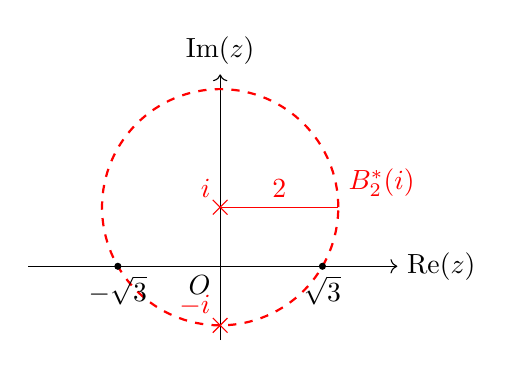
\begin{tikzpicture}[scale=.75]
				\draw[->] (-3.25,0) -- (3,0) node[right] {$\operatorname{Re}(z)$};
				\draw[->] (0,-1.25) -- (0,3.25) node[above] {$\operatorname{Im}(z)$};
				\draw[dashed,thick,red] (2,1) arc (0:360:2) node[above right] {$B_2^*(i)$};
				\node[below left] at (0,0) {$O$};
				\node[above left, red] at (0,1) {$i$};
				\node[above left, red] at (0,-1) {$-i$};
				\draw[fill=black] ({sqrt(3)},0) circle (0.05) node[below] {$\sqrt{3}$};
				\draw[fill=black] (-{sqrt(3)},0) circle (0.05) node[below] {$-\sqrt{3}$};
				\draw[red, mark size=5pt] plot[mark=x] coordinates{(0,1)};
				\draw[red, mark size=5pt] plot[mark=x] coordinates{(0,-1)};
				\draw[red] (0,1) -- (2,1) node[midway, above] {$2$};
				\end{tikzpicture}
			\end{center} Note that $0<\abs{z-i}<2\implies 0<\displaystyle\frac{\abs{z-i}}{2}<1$.
			\begin{align*}
				f(z)=\frac{1}{z^2+1}&=\frac{1}{z-i}\cdot\frac{1}{z+i}\\
				&=\frac{1}{z-i}\cdot\frac{1}{2i+z-i}\\
				&=\frac{1}{z-i}\cdot\frac{1/2i}{1-\of{-\displaystyle\frac{z-i}{2i}}}\\
				&=\frac{1}{z-i}\cdot\frac{1}{2i}\cdot\left[1+\of{\frac{z-i}{-2i}}+\of{\frac{z-i}{-2i}}^2+\of{\frac{z-i}{-2i}}^3+\cdots\right]\quad\because\abs{\frac{z-i}{-2i}}=\frac{\abs{z-i}}{2}<1\\
				&=\frac{1}{2i}(z-i)^{-1}+\frac{1}{2i(-2i)}+\frac{1}{2i(-2i)^2}(z-i)+\frac{1}{2i(-2i)^3}(z-i)^2+\cdots\\
				&=\frac{1}{2i}(z-i)^{-1}+\sum_{n=0}^\infty\frac{(-1)^{n+1}}{(2i)^{n+2}}(z-i)^n.
			\end{align*}
			\item Let $\abs{z}<1$ then \begin{align*}
				f(z)=\frac{e^z}{1-z}&=\of{1+z+\frac{1}{2!}z^2+\frac{1}{3!}z^3+\cdots}\of{1+z+z^2+z^3+\cdots}\\
				&=1+z+\frac{1}{2!}z^2+\frac{1}{3!}z^3+\frac{1}{4!}z^4+\cdots\\
				&\hspace{6mm}+z+z^2+\frac{1}{2!}z^3+\frac{1}{3!}z^4+\cdots\\
				&\hspace{12mm}+z^2+z^3+\frac{1}{2!}z^4+\cdots\\
				&=\frac{1}{0!}+\of{\frac{1}{1!}+\frac{1}{0!}}z+\of{\frac{1}{2!}+\frac{1}{1!}+\frac{1}{0!}}z^2+\of{\frac{1}{3!}+\frac{1}{2!}+\frac{1}{1!}+\frac{1}{0!}}z^3+\cdots\\
				&=\sum_{n=0}^\infty\of{\sum_{k=0}^n\frac{1.}{k!}z^n}.
			\end{align*}
			\item Let $z\neq 0$ then \begin{align*}
				f(z) = z\cos\of{\frac{1}{z}}&=z\cdot\left[1-\frac{1}{2!}\of{\frac{1}{z}}^2+\frac{1}{4!}\of{\frac{1}{z}}^4-\frac{1}{6!}\of{\frac{1}{z}}^6+\cdots\right]\\
				&=z-\frac{1}{2!}\of{\frac{1}{z}}+\frac{1}{4!}\of{\frac{1}{z}}^3-\frac{1}{6!}\of{\frac{1}{z}}^5+\cdots\\
				&=\sum_{n=0}^\infty\frac{(-1)^n}{(2n)!}z^{-(2n-1)}.
			\end{align*}
		\end{enumerate}
	\end{proof}
	\vspace{8pt}
	
	\begin{tcolorbox}[colback=white,colframe=white,arc=5pt,title={\color{black}\bf $\bullet$ Series Expansion of a Complex Function III}]
		Represent the function \[
		f(z)=\frac{1}{(z-1)(z-2)}
		\] in the form of $\sum_{n=-\infty}^\infty c_n(z-z_0)^n$ in each of the following regions with respect to the given $z_0$.
		\begin{enumerate}
			\item[(1)] $0<\abs{z-1}<1$,\quad $z_0=1$\hspace{24mm} (2) $1<\abs{z}<2$,\quad $z_0=0$
			\item[(3)] $\abs{z}<1$,\quad $z_0=0$\hspace{36mm} (4) $\abs{z}>2$,\quad $z_0=0$
		\end{enumerate}
		\begin{center}
			\begin{tikzpicture}[scale=.75]
			\draw[->] (-3.25,0) -- (3,0) node[right] {$\operatorname{Re}(z)$};
			\draw[->] (0,-1.25) -- (0,3.25) node[above] {$\operatorname{Im}(z)$};
			\foreach \i in {-1,1,2}
			\draw[] (.1,\i)--(-.1,\i) node[left] {$\i i$};
			\draw[dashed,thick,blue] (2,0) arc (0:360:1) node[above right] {$(1)$};
			%\node[below left] at (0,0) {$O$};
			%\draw[fill=black] ({sqrt(3)},0) circle (0.05) node[below] {$\sqrt{3}$};
			%\draw[fill=black] (-{sqrt(3)},0) circle (0.05) node[below] {$-\sqrt{3}$};
			\draw[red, mark size=2.5pt] plot[mark=x] coordinates{(1,0)} node[below] {$1$};
			\draw[red, mark size=2.5pt] plot[mark=x] coordinates{(2,0)} node[below] {$2$};
			%\node[above left, red] at (1,0) {$1$};
			%\node[above left, red] at (2,0) {$2$};
			%\draw[red] (0,1) -- (2,1) node[midway, above] {$2$};
			\end{tikzpicture}
		\end{center}
	\end{tcolorbox}
	\begin{proof}[\sol]
		\begin{enumerate}[(1)]
			\item \begin{align*}
			f(z)=\frac{1}{z-1}\cdot\frac{1}{z-2}&=\frac{1}{z-1}\cdot\frac{-1}{1-(z-1)}\\
			&=\frac{-1}{z-1}\of{1+(z-1)+(z-1)^2+\cdots}\quad\because\abs{z-1}<1\\
			&=-(z-1)^{-1}+(-1)+(-1)(z-1)+(-1)(z-1)^2+\cdots\\
			&=-(z-1)^{-1}+\sum_{n=0}^\infty(-1)(z-1)^n.
			\end{align*}
			\item Note that $\displaystyle f(z)=\frac{-1}{z-1}+\frac{1}{z-2}$. Then \[
			\begin{cases}
			\frac{-1}{z-1}=\frac{-1/z}{1-1/z}=-\frac{1}{z}\of{1+\of{\frac{1}{z}}+\of{\frac{1}{z}}^2+\cdots} &\because\abs{z}>1,\\
			\\
			\frac{1}{z-2}=\frac{-1/2}{1-z/2}=-\frac{1}{2}\of{1+\of{\frac{z}{2}}+\of{\frac{z}{2}}^2+\cdots} &\because\abs{z}<2.
			\end{cases}
			\] Thus \begin{align*}
			f(z)&=\of{-\frac{1}{z}-\frac{1}{z^2}-\frac{1}{z^3}-\cdots}+\of{-\frac{1}{2}-\frac{z}{2^2}-\frac{z^2}{2^3}+\cdots}=\sum_{n=1}^\infty(-1)z^{-n}+\sum_{n=0}^\infty\frac{-1}{2^{n+1}}z^n.
			\end{align*}
			\item Note that $\displaystyle f(z)=\frac{-1}{z-1}+\frac{1}{z-2}$. Then \[
			\begin{cases}
			\frac{-1}{z-1}=\frac{1}{1-z}=1+z+z^2+z^3+\cdots &\because\abs{z}<1,\\
			\\
			\frac{1}{z-2}=\frac{-1/2}{1-z/2}=-\frac{1}{2}\of{1+\of{\frac{z}{2}}+\of{\frac{z}{2}}^2+\cdots} &\because\abs{\frac{z}{2}}<\frac{1}{2}<1.
			\end{cases}
			\] Thus \begin{align*}
			f(z)&=\of{1+z+z^2+z^3+\cdots}+\of{-\frac{1}{2}-\frac{z}{2^2}-\frac{z^2}{2^3}-\cdots}\\
			&=\of{1-\frac{1}{2}}+\of{1-\frac{1}{2^2}}z+\of{1-\frac{1}{2^3}}z^2+\cdots\\
			&=\sum_{n=0}^\infty\of{1-\frac{1}{2^{n+1}}}z^n.
			\end{align*}
			\item Note that $\displaystyle f(z)=\frac{-1}{z-1}+\frac{1}{z-2}$. Then \[
			\begin{cases}
			\frac{-1}{z-1}=\frac{-1/z}{1-1/z}=-\frac{1}{z}\of{1+\of{\frac{1}{z}}+\of{\frac{1}{z}}^2+\cdots} &\because\abs{\frac{1}{z}}<\frac{1}{2}<1,\\
			\\
			\frac{1}{z-2}=\frac{1/z}{1-2/z}=\frac{1}{z}\of{1+\of{\frac{2}{z}}+\of{\frac{2}{z}}^2+\cdots} &\because\abs{\frac{2}{z}}<1.
			\end{cases}
			\] Thus \begin{align*}
			f(z)&=\of{-\frac{1}{z}-\frac{1}{z^2}-\frac{1}{z^3}-\cdots}+\of{\frac{1}{z}+\frac{2}{z^2}+\frac{2^2}{z^3}+\cdots}\\
			&=(-1+2^0)z^{-1}+(-1+2^1)z^{-2}+(-1+2^2)z^{-3}+\cdots\\
			&=\sum_{n=0}^\infty\of{2^n-1}z^{-(n+1)}.
			\end{align*}
		\end{enumerate}
	\end{proof}
	
	\begin{tcolorbox}[colback=white,colframe=white,arc=5pt,title={\color{black}\bf $\bullet$ Residue}]
		Find $\displaystyle \res\left[\frac{2z+4}{z^2-1},1\right]$. 
	\end{tcolorbox}
	\begin{proof}[\sol]
		Consider $0<\abs{z-1}<2$. \begin{align*}
		\frac{2z+4}{z^2-1}&=\frac{2z+4}{(z-1)(z+2)}\\
		&=\frac{2w+6}{w(w+2)}\quad w:=z-1,\ \ie,\ 0<\abs{w}<2 \\
		&=\of{\frac{2w+6}{w}}\cdot\of{\frac{1}{2-(-w)}}\\
		&=\of{2+\frac{6}{w}}\cdot\of{\frac{1/2}{1-(-w/2)}}\\
		&=\of{2+\frac{6}{w}}\cdot\frac{1}{2}\cdot\of{1+(-w/2)+(-w/2)^2+\cdots}\quad\because\abs{\frac{w}{2}}<1\\
		&=\of{1+\frac{3}{w}}\of{1+(-w/2)+(-w/2)^2+\cdots}\\
		&=\cdots+3w^{-1}+\cdots\\
		&=\cdots+3(z-1)^{-1}+\cdots.
		\end{align*}
		Thus $\displaystyle\res\left[\frac{2z+4}{z^2-1},1\right]=3.$
	\end{proof}
	\vspace{8pt}
	\begin{tcolorbox}[colback=white,colframe=black,arc=5pt,title={\color{white}\bf Classification of Singularities}]
		\begin{enumerate}[(1)]
			\item Let $f:D\to\C$. $z_0\in\C$ is \[
			\begin{cases}
			\text{Analystic Point}\\
			\\
			\text{Singularity}\begin{cases}
			\text{Isolated Singularity}
			\begin{cases}
			\text{Removable Singularity}\iff\exists\lim\limits_{z\to z_0} f(z)\\
			\\
			\text{Pole of order $k\geq 1$}\iff\exists\lim\limits_{z\to z_0}(z-z_0)^kf(z)\neq 0\\
			\\
			\text{Essential Singularity}
			\end{cases}
			\\
			\\
			\text{Non-isolated Singularity}
			\end{cases}
			\end{cases}
			\]
			\item The classification order of isolated singularities: \[
			\text{Isolated Singularity}?\longrightarrow\text{Removable Singularity}?\longrightarrow\text{Pole of Order $k$}?\longrightarrow\text{Essential Singularity}?.
			\]
		\end{enumerate}
	\end{tcolorbox}

	\begin{tcolorbox}[colback=white,colframe=white,arc=5pt,title={\color{black}\bf $\bullet$ Classification of Singularities I}]
		Classify the singularity at the isolated singularity $z_0$ of the following function $f$:
		\begin{enumerate}[(1)]
			\item $\displaystyle f(z)=\frac{\sin^2z}{z^2\cos z}$,\quad $z_0=0$
			\item $\displaystyle f(z)=\frac{1-e^{z^2}}{\sin^2z\cos z}$,\quad $z_0=0$
			\item $\displaystyle f(z)=\frac{\cos z-1}{z^2\sin z}$,\quad $z_0=0$
			\item $\displaystyle f(z)=\frac{z^3e^z}{z^{10}-1}$,\quad $z_0=1$
			\item $\displaystyle f(z)=\frac{\sin z\cos z}{z^4}$,\quad $z_0=0$
			\item $\displaystyle f(z)=e^{\displaystyle\frac{1+2z}{z}}$,\quad $z_0=0$
		\end{enumerate}
	\end{tcolorbox}
	\begin{proof}[\sol]
		\begin{enumerate}[(1)]
			\item \[
			\lim\limits_{z\to 0}f(z)=\lim\limits_{z\to 0}\left[\of{\frac{\sin z}{z}}^2\frac{1}{\cos z}\right]=1.
			\] Thus $z_0=0$ is a removable singularity.
			\item \begin{align*}
			\lim\limits_{z\to 0}\frac{1-e^{z^2}}{\sin^2z\cos z}&=\lim\limits_{z\to 0}\frac{1-e^{z^2}}{\sin^2z}\\
			&=\lim\limits_{z\to 0}\frac{-2ze^{z^2}}{2\sin z\cos z}\quad\text{by L'Hôpital's rule}\\
			&=\lim\limits_{z\to 0}\left[-\of{\frac{1}{\sin z/z}}\cdot\frac{e^{z^2}}{\cos z}\right]\\
			&=-1.
			\end{align*}
			Thus $z_0=0$ is a removable singularity.
			\item \begin{align*}
			\lim\limits_{z\to 0}zf(z)=\lim\limits_{z\to 0}\frac{\cos z-1}{z\sin z}&=\lim\limits_{z\to 0}\frac{-\sin z}{\sin z+z\cos z}\\
			&=\lim\limits_{z\to 0}\frac{-\cos z}{\cos z+\cos z-z\sin z}\\
			&=-\frac{1}{2}\neq 0.
			\end{align*} Thus $z_0=0$ is a simple pole.
			\item \begin{align*}
			\lim\limits_{z\to 1}(z-1)f(z)=\lim\limits_{z\to 1}\frac{(z^4-z^3)e^z}{z^{10}-1}&=\lim\limits_{z\to 1}\frac{(z^4-z^3)e^z+(4z^3-3z^2)e^z}{10z^{9}}\\
			&=\frac{e}{10}\neq 0.
			\end{align*} Thus $z_0=1$ is a simple pole.
			\item \[
			\lim\limits_{z\to 0}z^3f(z)=\lim\limits_{z\to 0}\left[\of{\frac{\sin z}{z}}{\cos z}\right]=1\neq 0.
			\] Thus $z_0=0$ is a pole of order $3$.
			\item Note that \[
			\lim\limits_{\substack{x\to 0+\\ y=0}}e^{1/z}=\lim\limits_{x\to 0+}e^{1/x}=\infty\neq 0=\lim\limits_{x\to 0-}e^{1/x}=\lim\limits_{\substack{x\to 0-\\ y=0}}e^{1/z},
			\] and so $\not\exists\lim\limits_{z\to 0}e^{1/z}$. We claim that
			$\forall k\in\Z^+:\not\exists\lim\limits_{z\to 0} z^ke^{\frac{1}{z}}:$ let $k\in\Z^+$ then
			\begin{align*}
			\lim\limits_{\substack{x\to 0+\\ y=0}}z^ke^{1/z}&=\lim\limits_{\substack{x\to 0+\\ y=0}}z^k\left[1+\of{\frac{1}{z}}+\frac{1}{2!}\of{\frac{1}{z}}^2+\cdots\right]\\
			&=\lim\limits_{x\to 0+}x^k\left[1+\of{\frac{1}{x}}+\frac{1}{2!}\of{\frac{1}{x}}^2+\cdots\right]\\
			&\geq\lim\limits_{x\to 0+}\frac{x^k}{(k+1)!x^{k+1}}=\frac{1}{(k+1)!}\lim\limits_{x\to 0+}\frac{1}{x}=\infty.
			\end{align*} Thus $z_0=0$ is an essential singularity.
		\end{enumerate}
	\end{proof}
	\vspace{8pt}
	\begin{tcolorbox}[colback=white,colframe=white,arc=5pt,title={\color{black}\bf $\bullet$ Classification of Singularities II}]
		Find and classify all singularities of the following complex function.
		\begin{enumerate}[(1)]
			\item $\displaystyle f(z)=\frac{\cos z}{z^2}$
			\item $\displaystyle f(z)=\frac{z^2+3z-1}{z+2}$
			\item $\displaystyle f(z)=\frac{e^z}{(z-1)^3}$
			\item $\displaystyle f(z)=\frac{z+1}{(z^2+4)(z-1)^3}$
		\end{enumerate}
	\end{tcolorbox}
	\begin{proof}[\sol]
		\begin{enumerate}[(1)]
			\item The singularity is at $0$ and it is a pole of order $2$.
			\item The singularity is at $-2$ and it is a pole of order $1$ (that is, simple pole).
			\item The singularity is at $1$ and it is a pole of order $3$.
			\item The singularities are at $2i$, $-2i$, and $1$, each of which is a pole with orders $1$, $1$, and $3$, respectively.
		\end{enumerate}
	\end{proof}
	\vspace{8pt}
	\begin{tcolorbox}[colback=white,colframe=white,arc=5pt,title={\color{black}\bf \textcolor{red}{$\star$} Classification of Singularities III}]
		Let's assume the complex function $f:\C\setminus\set{0}\to\C$ is analytic in $\C\setminus\set{0}$ and it satisfies \[
		\abs{f(z)}\leq\abs{z}+\frac{1}{\sqrt{\abs{z}}}\quad(\forall z\in\C\setminus\set{0}).
		\] Show that $f$ has a removable singularity at $z=0$ and compute the value of $f''(i)$.
	\end{tcolorbox}
	\begin{proof}[\sol]
		content...
	\end{proof}
	
	\begin{tcolorbox}[colback=white,colframe=white,arc=5pt,title={\color{black}\bf $\bullet$ Series Expansion of a Complex Function III}]
		
	\end{tcolorbox}
	
	
	\newpage
	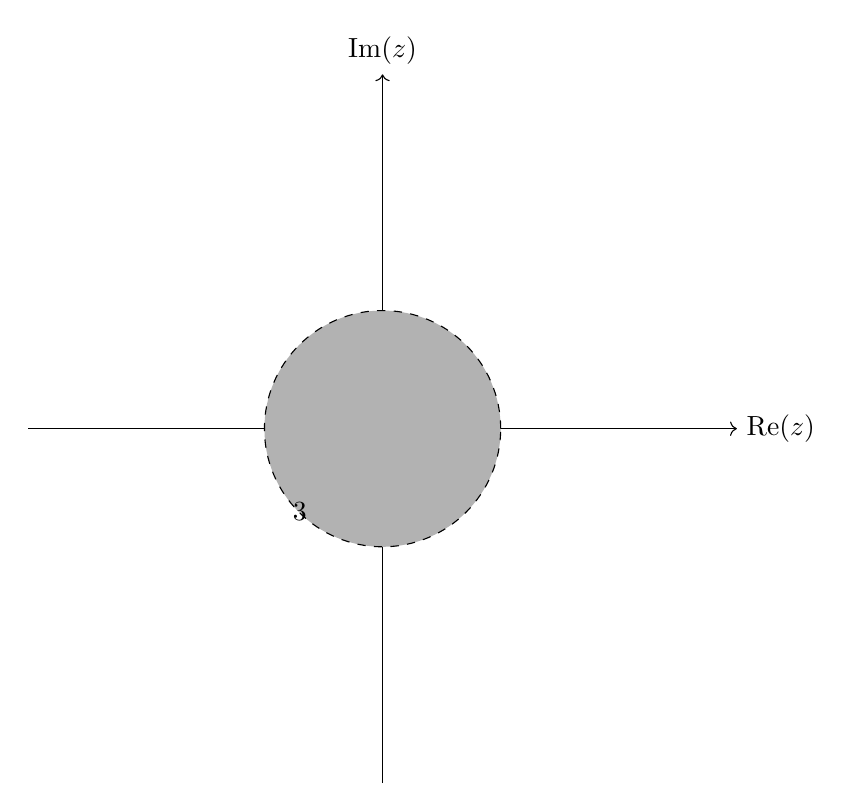
\begin{tikzpicture}[scale=1.5]
	% draw axis
	\draw[->] (-3,0) -- (3,0) node[right] {$\operatorname{Re}(z)$};
	\draw[->] (0,-3) -- (0,3) node[above] {$\operatorname{Im}(z)$};
	
	% (1) 0 < |z - 1| < 1
	%\draw[dashed, fill=gray!20] (1,0) circle (1);
	%\node at (1.5,0.5) {1};
	
	% (2) 1 < |z| < 2
	%\draw[dashed, fill=gray!40] (0,0) circle (2);
	%\draw[fill=white] (0,0) circle (1);
	%\node at (1.5,-1) {2};
	
	% (3) |z| < 1
	\draw[dashed, fill=gray!60] (0,0) circle (1);
	\node at (-0.7,-0.7) {3};
	
	% (4) |z| > 2
	% Outer region, can be represented with a larger circle
	%\draw[dashed] (0,0) circle (2.5);
	%\node at (-2,2) {4};
	\end{tikzpicture}
	\newpage
	\begin{enumerate}
		\item Express all complex solutions to the equation $z^6 - 64 = 0$ in the form $z = a + bi$.
		\begin{proof}[\sol]
			Let $z=re^{i\theta}$. Then \[
			z^6=r^6e^{i 6\theta}=64=2^6\implies\begin{cases}
			r = 2,\\
			6\theta = 2\pi\cdot k, \ie, \theta=\frac{k\pi}{3}\ \text{with}\ k\in\Z_{\geq 0}.
			\end{cases}
			\]
			\begin{center}
				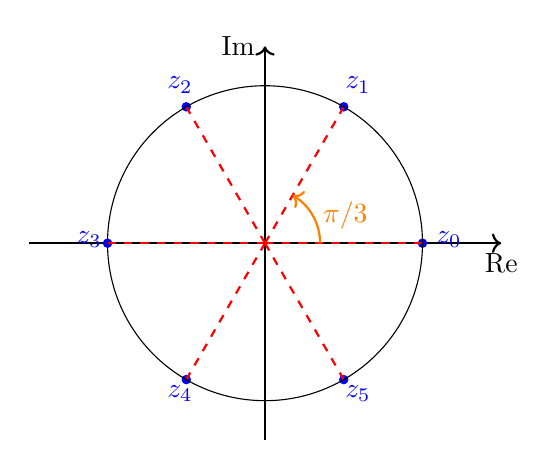
\begin{tikzpicture}
				\draw[thick,->] (-3.0,0) -- (3.0,0) node[below] {$\Re$};
				\draw[thick,->] (0,-2.5) -- (0,2.5) node[left] {$\Im$};
				
				\foreach \angle/\label [count=\k from 0] in {0/$z_0$, 60/$z_1$, 120/$z_2$, 180/$z_3$, 240/$z_4$, 300/$z_5$} {
					\coordinate (z\k) at (\angle:2);
					\draw[fill, blue] (z\k) circle (1.5pt) node[anchor={\angle-180}, shift={(0.05,0.05)}] {\label};
				}
				
				% draw radius
				\draw[dashed, thick, red] (0,0) -- (2,0) node[midway, above left, black] {};
				\draw[dashed, thick, red] (0,0) -- (1,{sqrt(3)}) node[midway, above left, black] {};
				\draw[dashed, thick, red] (0,0) -- (-1,{sqrt(3)}) node[midway, above left, black] {};
				\draw[dashed, thick, red] (0,0) -- (-2,0) node[midway, above left, black] {};
				\draw[dashed, thick, red] (0,0) -- (-1,-{sqrt(3)}) node[midway, above left, black] {};
				\draw[dashed, thick, red] (0,0) -- (1,-{sqrt(3)}) node[midway, above left, black] {};
				
				\draw[->, thick, orange] (.7,0) arc (0:60:.7) node[midway, right, orange] {$\pi/3$};
				\draw (0,0) circle (2);
				\end{tikzpicture}
			\end{center}
			Thus, $z_k=2\exp\of{\frac{k}{3}\pi i}$ with $k\in\set{0,1,2,3,4,5}:$\begin{align*}
			z_0&=2\of{\cos 0+i\sin 0}=2+0i,\\
			z_1&=2\of{\cos\of{\frac{\pi}{3}}+i\sin\of{\frac{\pi}{3}}}=1+\sqrt{3}i,\\
			z_2&=2\of{\cos\of{\frac{2\pi}{3}}+i\sin\of{\frac{\pi}{3}}}=-1+\sqrt{3}i,\\
			z_3&=2\of{\cos\pi+i\sin\pi}=-2+0i,\\
			z_4&=2\of{\cos\of{\frac{4\pi}{3}}+i\sin\of{\frac{4\pi}{3}}}=-1-\sqrt{3}i,\\
			z_5&=2\of{\cos\of{\frac{5\pi}{3}}+i\sin\of{\frac{5\pi}{3}}}=1-\sqrt{3}i.
			\end{align*}
			Note that: \begin{table}[ht!]
				\centering
				\begin{tabular}{c||c|c|c}
					\toprule
					Angle & $\sin(\theta)$ & $\cos(\theta)$ & $\tan(\theta)$ \\
					\midrule
					$0^\circ$ or $0$ & 0 & 1 & 0 \\
					$30^\circ$ or ${\pi}/{6}$ & ${1}/{2}$ & ${\sqrt{3}}/{2}$ & ${\sqrt{3}}/{6}$ \\
					$45^\circ$ or ${\pi}/{4}$ & ${1}/{\sqrt{2}}$ & ${1}/{\sqrt{2}}$ & 1 \\
					$60^\circ$ or ${\pi}/{3}$ & ${\sqrt{3}}/{2}$ & ${1}/{2}$ & $\sqrt{3}$ \\
					$90^\circ$ or ${\pi}/{2}$ & 1 & 0 & undefined \\
					$120^\circ$ or ${2\pi}/{3}$ & ${\sqrt{3}}/{2}$ & $-{1}/{2}$ & $-\sqrt{3}$ \\
					$135^\circ$ or ${3\pi}/{4}$ & ${1}/{\sqrt{2}}$ & $-{1}/{\sqrt{2}}$ & -1 \\
					$150^\circ$ or ${5\pi}/{6}$ & ${1}/{2}$ & $-{\sqrt{3}}/{2}$ & ${\sqrt{3}}/{3}$ \\
					$180^\circ$ or $\pi$ & 0 & -1 & 0 \\
					\bottomrule
				\end{tabular}
				%\caption{Special angles and their sine, cosine, and tangent values}
			\end{table}\\
		\end{proof}
		\vspace{8pt}
		\item Determine whether the following functions are differentiable and holomorphic at $z = 0$.
		\begin{enumerate}
			\item[(a)] $f\of{z}=f\of{x+iy}=\of{x+2y}+i\of{2x+y}$
			\item[(b)] $f\of{z}=\abs{z}^2+z$
			\item[(c)] $f\of{z}=f\of{x+iy}=e^x\cos y+ie^x\sin y$
			\item[(d)] $\displaystyle f\of{z}=f\of{x+iy}=\begin{cases}\displaystyle
			\frac{2x^3-3y^3}{2x^2+3y^2}+i\frac{2x^3+3y^3}{2x^2+3y^2} &:z\neq 0,\\
			0 &:z= 0.
			\end{cases}$
		\end{enumerate}
		\begin{proof}[\sol]
			Note that \begin{align*}
			\text{Complex-differentiable}&\Rightarrow\text{CR-Eq}\\
			\text{Complex-differentiable}&\Leftarrow\text{CR-Eq and $C^1$}\\
			\end{align*}\begin{enumerate}
				\item[(a)] Let $\begin{cases}
				u(x,y)=x+2y,\\
				v(x,y)=2x+y.
				\end{cases}$ Then \[
				u_x=1,\quad u_y=2,\quad v_x=2,\quad\text{and}\quad v_y=1.
				\] Thus $u_x=v_y$ but $u_y\neq -v_x$, that is, it does not hold CR-eqs. Thus $f$ is non-differentiable, and so not holomorphic. 
				\vspace{4pt}
				\item[(b)] Let $z=x+iy$ then $f\of{z}=x^2+y^2+(x+iy)$. Define $\begin{cases}
				u(x,y):=x^2+x+y^2,\\
				v(x,y):=y.
				\end{cases}$ Then \[
				u_x=2x+1,\quad u_y=2y,\quad v_x=0,\quad\text{and}\quad v_y=1.
				\] And so \begin{align*}
				u_x=v_y&\implies 2x+1=1\implies 2x=0,\\
				u_y=-v_x&\implies 2y=0.
				\end{align*} Thus $f$ is differentiable at $z=0$ only. It is not holomorphic.
				\vspace{4pt}
				\item[(c)] Let $\begin{cases}
				u(x,y)=e^x\cos y,\\
				v(x,y)=e^x\sin y
				\end{cases}$ then \[
				u_x=e^x\cos y,\quad u_y=-e^x\sin y,\quad v_x=e^x\sin y,\quad\text{and}\quad v_y=e^x\cos y.
				\] Since $u_x=v_y$ and $u_y=-v_x$, a function $f$ satisfies CR-Eqs and $C^1$. Thus $f$ is differentiable on $\C$ and holomorphic in $\C$. And \[
				f'\of{z}=u_x+iv_x=e^x\cos y+ie^x\sin y=e^{x+iy}=e^z.
				\]
				\vspace{4pt}
				\item[(d)] Note that \textbf{HW\#1}.
			\end{enumerate}
		\end{proof}
		\newpage
		\item For the curve $C:z(t) = 3 + 3e^{it}$ with $0\leq t\leq\pi$, find the $\displaystyle\int_C\conjugate{z}dz$.
		\begin{center}
			\begin{tikzpicture}[scale=1.2]
			\draw[->] (-1,0) -- (7,0) node[right] {$\operatorname{Re}(z)$};
			\draw[->] (0,-1) -- (0,4) node[above] {$\operatorname{Im}(z)$};
			\draw[thick,red] (6,0) arc (0:180:3);
			\node[below left] at (0,0) {$O$};
			\node[below right] at (3,0) {$3$};
			\node[below right] at (6,0) {$6$};
			\node[above left, red] at (3,3) {$D$};
			\node[above left] at (0,3) {$3i$};
			\draw[fill=black] (3,0) circle (0.05);
			\draw[fill=black] (6,0) circle (0.05);
			\draw[fill=black] (0,0) circle (0.05);
			\draw[fill=black] (0,3) circle (0.05);
			\end{tikzpicture}
		\end{center}
		\begin{proof}[\sol]
			Let $\tilde{C}$ be a straight joining origin to $(0,6)$. Define $D:=C+\tilde{C}$. Then \[
			\int_{C+\tilde{C}}\conjugate{z}dz=2i\cdot\of{\text{Area of semi-circle}}=2i\cdot\frac{9\pi}{2}=9\pi i.
			\] Since $\int_{\tilde{C}}\conjugate{z}dz\overset{z(t)=t}{=}\int_0^6\conjugate{t}dt=\int_0^6 tdt=\frac{1}{2}t^2\bigg|_0^6=18$, we have \[
			\int_C\conjugate{z}dz=\int_{C+\tilde{C}}\conjugate{z}dz-\int_{\tilde{C}}\conjugate{z}dz=9\pi -18.
			\]
		\end{proof}
		\vspace{8pt}
		\item Let $C$ be a straight line joining $z_1=0$ to $z_2=1+i$. For $f\of{z}=3z^2+4iz$, find $\int_C f\of{z}dz$.
		\begin{proof}[\sol]
			Note that \[
			f\of{z}=3z^2+4iz=\frac{d}{dz}\left[z^3+2iz^2\right].
			\] Let $F\of{z}:=z^3+2iz^2$. Then \begin{align*}
			\int_Cf\of{z}dz=\int_0^{1+i}f\of{z}dz=F\of{1+i}-F\of{0}&=\of{1+i}^3-2i(1+i)^2-0\\
			&=1+3i+3i^2+i^3-2i(1+2i+i^2)\\
			&=-2+2i+(-2i+4+2i)\\
			&=2+2i.
			\end{align*}
		\end{proof}
		\newpage
		\item Define a principal value of complex exponent as follows: \[
		\pv z^\alpha:=\exp\of{a\Log z}.
		\] Find $\abs{\pv\of{1-i}^{1+i}}$.
		\begin{proof}[\sol]
			Note that \begin{align*}
			\pv (1-i)^{1+i}&=\exp\left[(1+i)\Log(1-i)\right]\\
			&=\exp\left[(1+i)\set{\ln\abs{1-i}+i\Arg\of{1-i}}\right]\\
			&=\exp\left[(1+i)\of{\ln\sqrt{2}-\frac{\pi}{4}i}\right]\\
			&=\exp\left[\of{\ln\sqrt{2}+\frac{\pi}{4}}+i\of{\ln\sqrt{2}-\frac{\pi}{4}}\right].
			\end{align*} Thus, \begin{align*}
			\abs{\pv(1-i)^{1+i}}&=\abs{\exp\of{\ln\sqrt{2}+\frac{\pi}{4}}}\abs{\exp\left[i\of{\ln\sqrt{2}-\frac{\pi}{4}}\right]}\\
			&=\sqrt{2}\exp\of{\frac{\pi}{4}}\quad\because \abs{e^{i\theta}}=1.
			\end{align*}
		\end{proof}
		\vspace{8pt}
		\item Consider the complex function $h\of{z}$ defined as follows: \[
		h\of{z}=h\of{x+iy}=\of{x^3+3xy^2-3x}+i\of{y^3+3x^2y-3y}.
		\]\begin{itemize}
			\item[(a)] Show that $h\of{z}$ is differentiable at all points on $x$-axis.
			\item[(b)] Find all points where $h\of{z}$ is holomorphic.
		\end{itemize}
		\begin{proof}[\sol]
			\begin{itemize}
				\item[(a)]
				Let $\begin{cases}
				u(x,y)=x^3+3xy^2-3x\\
				v(x,y)=y^3+3x^2y-3y
				\end{cases}$ then \[
				\begin{cases}
				u_x=3x^2+3y^2-3\\
				u_y=6xy
				\end{cases},\quad
				\begin{cases}
				v_x=6xy\\
				v_y=3y^2+3x^2-3.
				\end{cases}
				\] Thus, \[\begin{cases}
				u_x=v_y&\\
				u_y=-v_x &\text{if $y=0$ or $x=0$}
				\end{cases}
				\] Therefore, $h$ is complex differentiable on $x=0$ ($y$-axis) or $y=0$ ($x$-axis).
				\vspace{4pt}
				\item[(b)] Consider a $\delta$-neighborhood $N_{\delta>0}(z_0)=\set{z:\abs{z-z_0}<\delta}$ of a point $z_0=x_0+i\cdot 0$ on $y=0$. Thus there is no holomorphic point.
			\end{itemize}
		\end{proof}
		
		\newpage
		\item The curve $C$ is the unit circle $z(t) = e^{it}$ for $0\leq t\leq 2\pi$. Calculate the following integral: \begin{enumerate}
			\item[(a)] $\displaystyle\int_C\frac{2z-10}{z^2-10z}dz$.
			\vspace{4pt}
			\item[(b)] $\displaystyle\int_C\frac{\sinh z}{z^4}dz$.
		\end{enumerate}
		\begin{proof}[\sol]
			Recall that Cauchy integral formula: \[
			f^{(n)}(z_0)=\frac{n!}{2\pi}\oint_C\frac{f\of{z}}{\of{z-z_0}^{n+1}}dz.
			\]
			\begin{itemize}
				\item[(a)] \begin{align*}
				\int_C\frac{2z-10}{z^2-10z}dz&=\oint_C\of{\frac{1}{z}+\frac{1}{z-10}}dz\\
				&=\oint_C\frac{1}{z}dz+\oint_C\frac{1}{z-10}dz\\
				&=2\pi i+0\quad\text{by Cauchy Integral Theorem and Cauchy-Gorusat Theorem}.
				\end{align*}
				\item[(b)] Let $f\of{z}=\sinh z$. Then \[
				f^{(3)}(0)=\frac{3!}{2\pi i}\oint_C\frac{\sinh z}{(z-0)^4}dz=\frac{3}{\pi i}\oint_C\frac{\sinh z}{z^4}dz.
				\] Since $f^{(3)}(z)=\cosh z\Rightarrow f^{(3)}(0)=1$, we have $\displaystyle\int_C\frac{\sinh z}{z^4}dz=\frac{\pi i}{3}$.
			\end{itemize}
		\end{proof}
		\vspace{8pt}
		\item Let the two curves $C_R$ and $C_\rho$ in the complex plane be positively oriented semicircles, defined as follows:
		\[
		C_R: z(t) = Re^{it},\quad  C_\rho: z(t) = \rho e^{it},\quad \of{0\leq t\leq\pi}.
		\] Let the complex function $\displaystyle f(z) = \frac{z^2}{\of{z^2+1}^2}$. 
		\begin{center}
			\begin{tikzpicture}
			\draw[thick,->] (-6.0,0) -- (6.0,0) node[below] {$\Re$};
			\draw[thick,->] (0,-.5) -- (0,5) node[left] {$\Im$};
			
			\node[below] at (2,0) {$\rho$};
			\node[below] at (4,0) {$R$};
			\node[below] at (-2,0) {$-\rho$};
			\node[below] at (-4,0) {$-R$};
			\draw[fill=red] (2,0) circle (0.05);
			\draw[fill=red] (4,0) circle (0.05);
			\draw[fill=red] (-2,0) circle (0.05);
			\draw[fill=red] (-4,0) circle (0.05);
			
			\draw[->, thick, red] (2,0) arc (0:180:2) node[above left, black] {$C_\rho$};
			\draw[->, thick, red] (4,0) arc (0:180:4) node[above left, black] {$C_R$};
			%\draw[->, thick, red] (2,0) arc (0:90:2)
			%\draw[->, thick, red] (4,0) arc (0:90:4)
			%\draw (0,0) circle (2);
			\end{tikzpicture}
		\end{center}
		\vspace{4pt}
		\begin{enumerate}
			\item[(a)] Prove the following inequality when $R=3$: \[
			\abs{\int_{C_R}f\of{z}dz}<\frac{1}{2}\pi.
			\] As the radius $R$ approaches infinity $\of{R\to\infty}$, where does the integral value converge?
			\item[(b)] Prove the following inequality when $\rho = 1/3$:
			\[
			\abs{\int_{C_\rho}f\of{z}dz}<\frac{1}{16}\pi.
			\] As the radius $\rho$ approaches zero $\of{\rho\to 0}$, where does the integral value converge?
		\end{enumerate}
		\begin{proof}[\sol]
			\begin{enumerate}
				\item[(a)] For $\abs{z}=3$, we have $\abs{z^2+1}\geq\abs{\abs{z}^2-1}=8$. Then \[
				\abs{f\of{z}}=\frac{\abs{z}^2}{\abs{z^2+1}^2}\leq\frac{9}{64}.
				\] Thus \[
				\abs{\int_{C_R}f\of{z}dz}\leq\max_{z\in C_R}\abs{f\of{z}}\int_{C_R}\abs{dz}\leq\frac{9}{64}\cdot3\pi=\frac{27}{64}\pi<\frac{1}{2}\pi.
				\] Suppose that $R\to\infty$ then \[
				\abs{\int_{C_R}f\of{z}dz}\leq\frac{R^2}{\of{R^2-1}^2}\cdot\pi R=\frac{\pi R^3}{\of{R^2-1}^2}\to 0.
				\]
				\vspace{4pt}
				\item[(b)] For $\abs{z}=1/3$, we have $\abs{z^2+1}\geq 1-\abs{z}^2=1-\rho^2=8/9$. Then \[
				\abs{f\of{z}}=\frac{\abs{z}^2}{\abs{z^2+1}^2}\leq\frac{\rho^2}{(1-\rho^2)^2}=\frac{1/9}{\of{8/9}^2}=\frac{9}{64}.
				\] Thus, \[
				\abs{\int_{C_\rho}f\of{z}dz}\leq\max_{z\in C_\rho}\abs{f\of{z}}\int_{C_\rho}\abs{dz}\leq\frac{9}{64}\cdot\frac{1}{3}\pi=\frac{3}{64}\pi<\frac{1}{16}\pi.
				\] Suppose that $\rho\to 0$ then \[
				\abs{\int_{C_\rho}f\of{z}dz}\leq\frac{\rho^2}{\of{1-\rho^2}^2}\cdot\pi \rho=\frac{\pi \rho^3}{\of{1-\rho^2}^2}\to \frac{0}{1}=0.
				\]
			\end{enumerate}
		\end{proof}
		
		\newpage
		\item Show that an entire function $f$ becomes a constant function if it satisfies the following condition: \[
		\abs{f\of{z}}\geq 1,\quad z\in\C.
		\]
		\begin{proof}[\sol]
			We use Liouville's theorem: ``bounded and entire $\Rightarrow$ constant''. Define an entire function \[
			g\of{z}:=\frac{1}{f\of{z}}.
			\] Then $\abs{g\of{z}}=\frac{1}{\abs{f\of{z}}}\leq 1$, \ie, $g$ is bounded. By Liouville's theorem, $g$ be a constant function, and hence $f$ be a constant.
		\end{proof}
		\vspace{8pt}
		\item For an entire function $f$ satisfying the following condition: \[
		\abs{f\of{z}}\leq 3\abs{z},\quad z\in\C,
		\] \begin{enumerate}
			\item[(a)] Show that $f^{(n)}(z) = 0$ ($n\geq 2$) for all points $z$.
			\item[(b)] Demonstrate that a function satisfying this condition is a linear polynomial, \ie, $f(z) = az + b$.
		\end{enumerate}\begin{proof}[\sol]
			\begin{itemize}
				\item[(a)] By the Cauchy integral formula, \begin{align*}
				\abs{f^{(2)}\of{z_0}}=\abs{\frac{2!}{2\pi i}\oint_{C_R}\frac{f\of{z}}{\of{z-z_0}^3}dz}&=\frac{1}{\pi}\abs{\oint_{C_R}\frac{f(z)}{(z-z_0)^3}dz}\\
				&\leq\frac{1}{\pi}\cdot\max_{z\in C_R}\frac{\abs{f\of{z}}}{\abs{z-z_0}^3}\cdot 2\pi R\\
				&\leq 2R\cdot\frac{3R}{\of{R-\abs{z_0}}^3}\\
				&=\frac{6R}{\of{R-\abs{z_0}}^3}\\
				&\to 0\quad\text{as $R\to\infty$}.
				\end{align*} Thus, $f^{(n)}=0$ for all $n\geq 2$.
				\vspace{4pt}
				\item[(b)] \[
				f^{(2)}(z)=0\implies f^{(1)}(z)=c\in\C\implies f(z)=az+b\ (\text{linear}).
				\]
			\end{itemize}
		\end{proof}
	\end{enumerate}
	
	
	\footer{Department of Information Security, Cryptography and Mathematics\\
	Collage of Science and Technology\\
	Kookmin University}
\end{document}
